% Created 2021-09-11 Sat 08:18
% Intended LaTeX compiler: xelatex
\documentclass[letterpaper]{article}
\usepackage{graphicx}
\usepackage{grffile}
\usepackage{longtable}
\usepackage{wrapfig}
\usepackage{rotating}
\usepackage[normalem]{ulem}
\usepackage{amsmath}
\usepackage{textcomp}
\usepackage{amssymb}
\usepackage{capt-of}
\usepackage{hyperref}
\usepackage[margin=1in]{geometry}
\usepackage{fontspec}
\usepackage{indentfirst}
\setmainfont[ItalicFont = LiberationSans-Italic, BoldFont = LiberationSans-Bold, BoldItalicFont = LiberationSans-BoldItalic]{LiberationSans}
\newfontfamily\NHLight[ItalicFont = LiberationSansNarrow-Italic, BoldFont       = LiberationSansNarrow-Bold, BoldItalicFont = LiberationSansNarrow-BoldItalic]{LiberationSansNarrow}
\newcommand\textrmlf[1]{{\NHLight#1}}
\newcommand\textitlf[1]{{\NHLight\itshape#1}}
\let\textbflf\textrm
\newcommand\textulf[1]{{\NHLight\bfseries#1}}
\newcommand\textuitlf[1]{{\NHLight\bfseries\itshape#1}}
\usepackage{fancyhdr}
\pagestyle{fancy}
\usepackage{titlesec}
\usepackage{titling}
\makeatletter
\lhead{\textbf{\@title}}
\makeatother
\rhead{\textrmlf{Compiled} \today}
\lfoot{\theauthor\ \textbullet \ \textbf{2021-2022}}
\cfoot{}
\rfoot{\textrmlf{Page} \thepage}
\titleformat{\section} {\Large} {\textrmlf{\thesection} {|}} {0.3em} {\textbf}
\titleformat{\subsection} {\large} {\textrmlf{\thesubsection} {|}} {0.2em} {\textbf}
\titleformat{\subsubsection} {\large} {\textrmlf{\thesubsubsection} {|}} {0.1em} {\textbf}
\setlength{\parskip}{0.45em}
\renewcommand\maketitle{}
\author{Albert Huang}
\date{\today}
\title{Axler 2.C Exercise 17}
\hypersetup{
 pdfauthor={Albert Huang},
 pdftitle={Axler 2.C Exercise 17},
 pdfkeywords={},
 pdfsubject={},
 pdfcreator={Emacs 27.2 (Org mode 9.4.4)}, 
 pdflang={English}}
\begin{document}

\maketitle

\section{Problem}
\label{sec:orga50a849}

\begin{quote}
Prove or give a counterexample:
\$\$
\begin{aligned}
\text{dim}(U_1+U_2+U_3)\\
=&\text{dim}\ U_1 + \text{dim}\ U_2 + \text{dim}\ U_3\\
&-\text{dim}(U_1 \cap U_2)-\text{dim}(U_1 \cap U_3) - \text{dim}(U_2 \cap U_3)\\
&+\text{dim}(U_1\cap U_2 \cap U_3)
\end{aligned}
\$\$
\end{quote}

\section{Reasoning}
\label{sec:org256fe42}

By Axler2.41 we know that

$$
\text{dim}(U_1 + U_2) = \text{dim}\ U_1 + \text{dim}\ U_2 - \text{dim}(U_1 \cap U_2)
$$

By applying this formula to itself, we find that

\$\$
\begin{aligned}
\text{dim}(U_1 + U_2 + U_3)\\
&= \text{dim}((U_1 + U_2) + U_3)\\
&= \text{dim}(U_1 + U_2) + \text{dim}\ U_3 - \text{dim}( (U_1+U_2) \cap U_3 )\\
&= \text{dim}\ U_1 + \text{dim}\ U_2 -\text{dim}(U_1 \cap U_2) + \text{dim}\ U_3 - \text{dim}( (U_1+U_2) \cap U_3 )
\end{aligned}
\$\$

To show that the lemma is true, we would have to show that

\$\$
\begin{aligned}
\cancel{\text{dim}\ U_1 + \text{dim}\ U_2 + \text{dim}\ U_3 -\text{dim}(U_1 \cap U_2)} &-\text{dim}(U_1 \cap U_3) - \text{dim}(U_2 \cap U_3) +\text{dim}(U_1\cap U_2 \cap U_3)\\=
\cancel{\text{dim}\ U_1 + \text{dim}\ U_2 -\text{dim}(U_1 \cap U_2) + \text{dim}\ U_3} &- \text{dim}( (U_1+U_2) \cap U_3 )
\end{aligned}
\$\$

and to provide a counterexample, we just need to find some \(U_1\), \(U_2\), \(U_3\) such that

$$
\text{dim}(U_1 \cap U_3) + \text{dim}(U_2 \cap U_3) - \text{dim}(U_1\cap U_2 \cap U_3) \neq \text{dim}( (U_1+U_2) \cap U_3 )
$$

\section{Counterexample}
\label{sec:org1a58688}

If we choose

\$\$
\begin{aligned}
U_1 = \left\{\begin{pmatrix}x\\0\end{pmatrix} : x \in \mathbb{R} \right\}\\
U_2 = \left\{\begin{pmatrix}0\\x\end{pmatrix} : x \in \mathbb{R} \right\}\\
U_3 = \left\{\begin{pmatrix}x\\x\end{pmatrix} : x \in \mathbb{R} \right\}\\
\end{aligned}
\$\$

then the graph of the subspaces looks like this:

\begin{center}
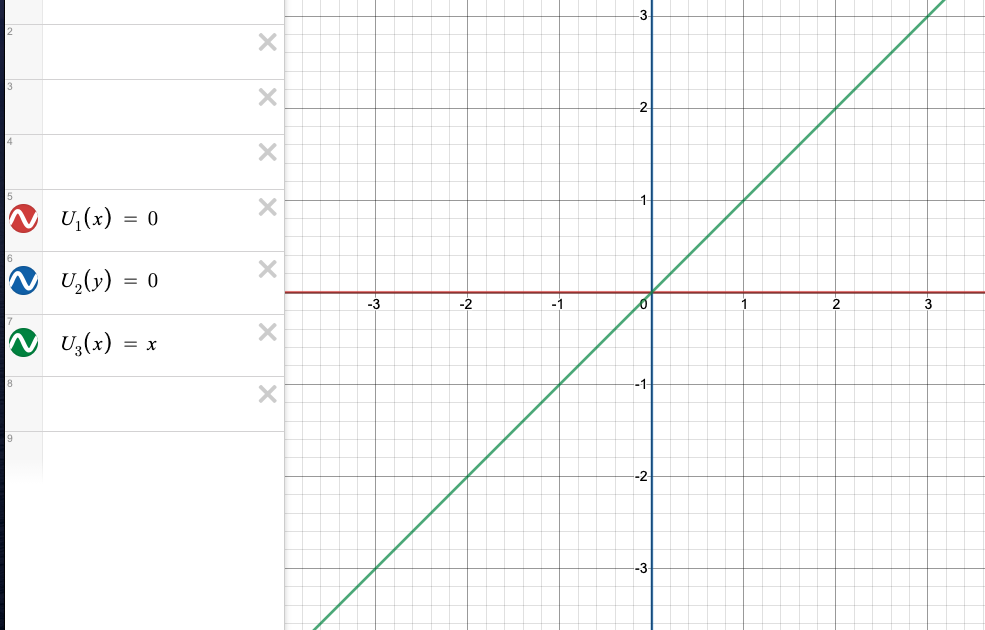
\includegraphics[width=.9\linewidth]{./KBe20math530retAxler2C17Subspaces.png}
\end{center}

and the dimesion of each intersection is \(0\) while the dimension of \((U_1+U_2) \cap U_3 = 2\). Thus, we have

\$\$
\begin{aligned}
\cancelto{0}{\text{dim}(U_1 \cap U_3)} + \cancelto{0}{\text{dim}(U_2 \cap U_3)} - \cancelto{0}{\text{dim}(U_1\cap U_2 \cap U_3)} \neq \text{dim}( (U_1+U_2) \cap U_3 )\\
\implies 0 \neq 2
\end{aligned}
\$\$

In summary, the sum of these subpsaces is \(\mathbb{R}^2\) and the dimension of the sum is 2, but
\$\$
\begin{aligned}
\text{dim}(U_1+U_2+U_3) = 2 \neq 3 = 1 + 1 + 1 - 0 - 0 - 0 + 0
\end{aligned}
\$\$
\end{document}
